\section{Versuchsaufbau/-durchführung}

\subsection{Versuchsaufbau}

Der normale und anomale Zeeman-Effekt soll mit Hilfe der roten (normaler Zeeman-Effekt)
und blauen (anomaler Zeeman-Effekt) Spektralinie einer $\ce{Cd}$-Lampe untersucht werden.
Das für die Energieaufspaltung benötigte Magnetfeld wird von einem Elektromagnet erzeugt.
Deshalb wird die Lampe zwischen die Polschuhe des Elektromagneten gestellt.
Das von der Lampe ausgehende Licht wird von einem optischen Aufbau gebündelt und aufgespaltet
in eine Lummer-Gehrcke Platte geleitet. Der optische Aufbau und der grundlegende Versuchsaufbau
sind in Abbildung \ref{fig: versuchsaufbau} skizziert.
Mit dem Linsensystem soll das Licht gebündelt und fokussiert werden.
Das auf das Geradenprisma gerichtete Licht, wird von diesem aufgespalten und anschließend von einem
weiteren Linsensystem auf die Lummer-Gehrcke Platte gebündelt.
\FloatBarrier
\begin{figure}[h]
  \centering
  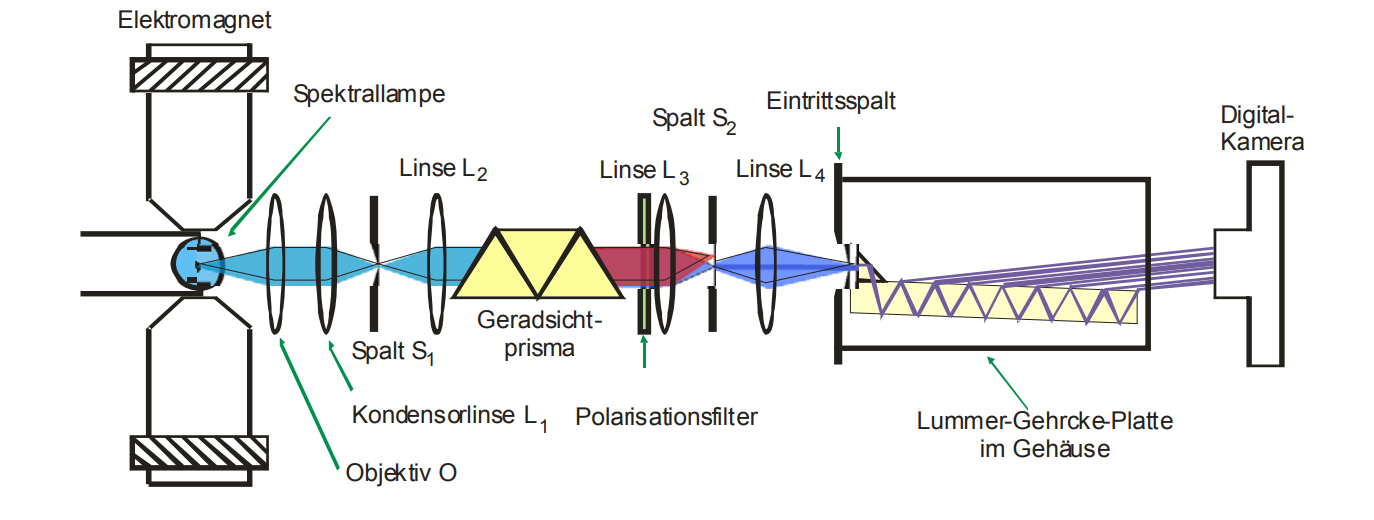
\includegraphics[width=0.85\textwidth]{pics/versuchsaufbau.png}
  \caption{Versuchsaufbau zur Untersuchung des Zeeman-Effektes \cite{anleitung27}.}
  \label{fig: versuchsaufbau}
\end{figure}
\FloatBarrier

Der in der Abbildung \ref{fig: versuchsaufbau} dargestellte Polarisationsfilter wird dazu genutzt, %Abbildung, dargestellte, genutzt,
die $\pi$ und $\sigma$ Übergänge zu unterscheiden. Das Verwenden einer Lummer-Gehrcke Platte
bietet sich immer dann an, wenn ein besonders hohes Auflösungsvermögen benötigt wird
und monochromatisches Licht untersucht werden soll.
Das Auflösungsvermögen kann mittels
\begin{equation}
  \label{eq: auflösungsvermoegen_lummer}
  A=\frac{L}{\lambda}(n(\lambda)^2-1)
\end{equation}
berechnet werden, hierbei ist L die Plattenlänge, $\lambda$ die Wellenlänge
des zu untersuchenden Lichtes und $n(\lambda)$ der wellenlängenabhängige
Brechungsindex der Platte. Mit Hilf eiens Prismas wird Licht in die Platte eingeleitet. %Hilfe eines ... in die
Das Licht wird innerhalb der Platte fast vollständig reflektiert, der transmittierte
Teil interferiert untereinander. Die Interferenz entsteht durch den Gangunterschied
der trasmistierten Lichtstrahlen (vgl. Abb. \ref{fig: lummer}). Ist der Gangunterschied
eines ganzzahliges vielfaches der Wellenlänge so wird konstruktive Interferenz beobachtet.
Wird monochromatisches Licht in die Lummer-Gehrcke Platte eingestrahlt, ist der
Gangunterschied der Interferenzstreifen gleich der Wellenlänge $\lambda$.
Ein beispielhafter Strahlengang in der Lummer-Gehrcke Platte ist in Abbildung \ref{fig: lummer} zu erkennen.
\FloatBarrier
\begin{figure}[h]
  \centering
  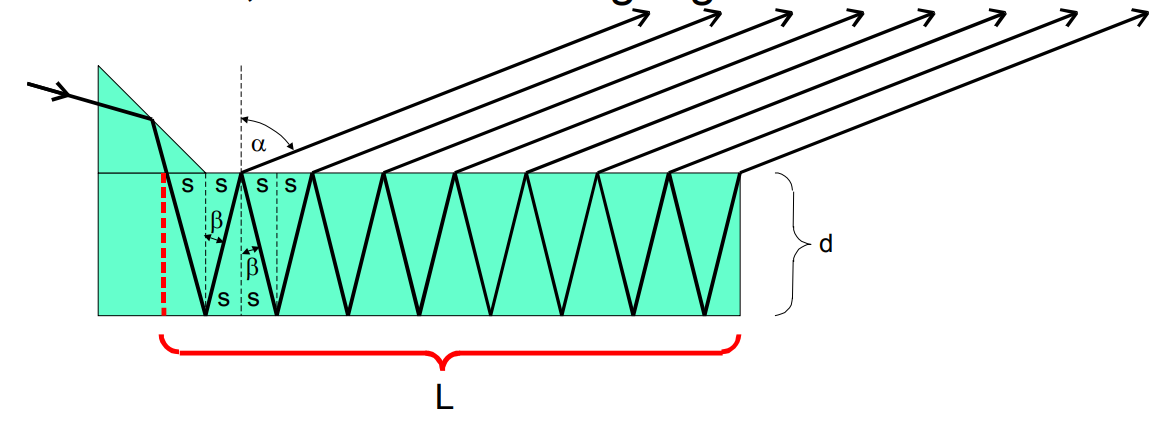
\includegraphics[width=0.7\textwidth]{pics/lummer.png}
  \caption{Aufbau einer Lummer-Gehrcke Platte \cite{anleitung27}.}
  \label{fig: lummer}
\end{figure}
\FloatBarrier
Zwei unterschiedliche Wellenlängen werden von einer Lummer-Gehrcke Platte bis zu
einer Längendifferenz von
\begin{equation}
  \label{eq: lummer_wellendif}
  \delta \lambda\ua{D}=\frac{\lambda^2}{2 d} \sqrt{\frac{1}{n^2-1}}
\end{equation}
unterscheidbar aufgelöst. Die Größe $\delta \lambda\ua{D}$ wird auch als Dispersionsgebiet
bezeichnet.

\subsection{Versuchsvorbereitung}

Im folgenden soll der Übergang  $^1P_1\leftrightarrow ^1\!\!D_2$ genauer betrachtet werden.
Das Termschema ist in Abbildung \ref{fig: termschema_rot} zu sehen. Die berechneten Landé-Faktoren %berechneten Landé
sind in Tabelle \ref{tab:Lande_rot} aufgelistet.

\FloatBarrier
\begin{figure}[h]
  \centering
  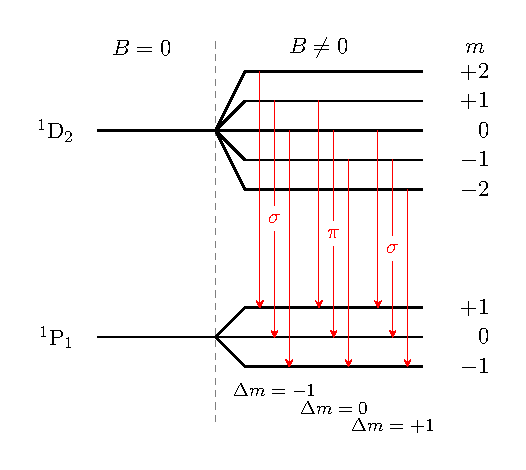
\includegraphics[width=0.6\textwidth]{pics/termschema_rot.pdf}
  \caption{Termschema für den Übergang $^1P_1\leftrightarrow ^1\!\!D_2$ \cite{luckyjosh}.}
  \label{fig: termschema_rot}
\end{figure}
\FloatBarrier
\FloatBarrier
\begin{table}
	\centering
  \caption{Landé-Faktoren für den Übergang $^1P_1\leftrightarrow ^1\!\!D_2$.  Berechnet mit Gleichung \eqref{eq:lande_faktor}.}
	\label{tab:Lande_rot}
	\begin{tabular}{cccccc}
		\toprule
		{} & \multicolumn{2}{c}{${}^1P_1$}  & \multicolumn{2}{c}{${}^1D_2$}  & $^1P_1\leftrightarrow ^1\!\!D_2$ \\
		\midrule
		 Übergang &   $m_1$  & $g_{1}$ & $m_2$ & $ g_2$  & $g_{12}$  \\
		\midrule
		& 2 & 1 & 1 & 1 & 1\\
		$\sigma$& 1 & 1 & 0 & 1 & 1\\
		& 0 & 1 & -1 & 1 & 1\\
		\midrule
		& 1 & 1 & 1 & 1 & 0\\
		$\pi$ & 0 & 1 & 0 & 1 & 0\\
		& -1 & 1 & -1 & 1 & 0\\
		\midrule
		& 0 & 1 & 1 & 1 & -1\\
		$\sigma$ & -1 & 1 & 0 & 1 & -1\\
		& -2 & 1 & -1 & 1 & -1\\\bottomrule
	\end{tabular}

\end{table}
\FloatBarrier
Der Übergang $^3S_1\leftrightarrow ^3\!\!P_1$ besitzt das in Abbildung \ref{fig: termschema_blau} gezeigte
Termschema. Die zugehörigen Landé-Faktoren sind in Tabelle \ref{tab:Lande_blau} zusehen. %Landé


\FloatBarrier
\begin{figure}[h]
  \centering
  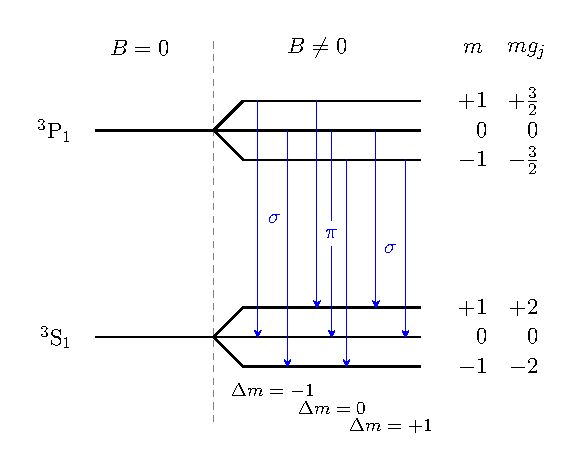
\includegraphics[width=0.6\textwidth]{pics/termschema_blau.pdf}
  \caption{Termschema für den Übergang $3S_1\leftrightarrow ^3\!\!P_1$ \cite{luckyjosh}.}
  \label{fig: termschema_blau}
\end{figure}
\FloatBarrier

\FloatBarrier
\begin{table}

  \caption{Landé-Faktoren für den Übergang $^3S_1\leftrightarrow ^3\!\!P_1$. Berechnet mit Gleichung \eqref{eq:lande_faktor}.} %Landé
	\label{tab:Lande_blau}
	\centering
  \renewcommand{\arraystretch}{1.2}
  \begin{tabular}{cccccc}
		\toprule
    & \multicolumn{2}{c}{${}^3S_1$}  & \multicolumn{2}{c}{${}^3P_2$} \\
		\midrule
    Übergang & $m_1$  & $g_{1}$ & $m_2$ & $ g_2$ & $g_{12}$\\
		\midrule
		$\sigma$ & +1 & 2 & 0 & $\frac{3}{2}$& 2\\
		& 0 & 2 & -1 & $\frac{3}{2}$ & $\frac{3}{2}$\\
		\midrule
		& +1 & 2 & +1 & $\frac{3}{2}$ & $\frac{1}{2}$\\
		$\pi$ & 2 & 2 & 0 & $\frac{3}{2}$ & 0 \\
		& -1 & 2 & -1 & $\frac{3}{2}$ & -$\frac{1}{2}$\\
		\midrule
		& 0 & 2 & 1 & $\frac{3}{2}$ & -$\frac{3}{2}$\\
		$\sigma$ & -1 & 2 & 0 & $\frac{3}{2}$& -2\\
		\bottomrule
	\end{tabular}
\end{table}
\FloatBarrier

Als abschließende Vorbereitung werden noch das Auflösungsvermögen und das Dispersionsgebiet
für die beiden Übergänge berechnet:
\begin{align}
\text{rotes Licht}\quad  \lambda&=\SI{643.8}{\nano\meter} \notag\\
   A(\SI{643.8}{\nano\meter})&\approx 209128.6, \quad \Delta \lambda(\SI{643.8}{\nano\meter})\approx\SI{4.98e-11}{\meter} \label{eq: auf_dis_rot} \\
\text{blaues Licht}  \quad \lambda&=\SI{480.0}{\nano\meter}\notag \\
 A(\SI{480.0}{\nano\meter})&\approx 285458, \quad \Delta \lambda(\SI{480.0}{\nano\meter})\approx \SI{2.7e-11}{\meter} \label{eq: auf_dis_blau}.
\end{align}


\subsubsection{Versuchsdurchführung}
Zunächst wird die optische Apparatur so eingestellt, dass Licht mit einer hohen Helligkeit %Zunächst, werden, dass
an der Lummer-Gehrcke Platte ankommt. Die einzelnen Spalten werden so angepasst, dass die %angepasst, dass
einzelnen Spektrallinien möglichst dünn und scharf abgebildet werden.

Anschließend wird der Elektromagnet kalibriert und auf Hystereseeffekte untersucht.
Dazu wird mittels einer Hall-Sonde die Magnetfeldstärke für Stromstärken
zwischen $\num{1}-\num{20}\,\si{\ampere}$ gemessen. Um gleichzeitig den Magnet auf Hysteresseeffekte zu untersuchen,
wird die Magnetfeldstärke auf einem aufsteigenden Ast ($I_i>I_j,\, i>j$) untersucht und einmal auf einem absteigenden ($I_i<I_j,\, i>j$).

Als Erstes wird rotes Licht $\lambda = \SI{643.8}{\nano\meter}$ untersucht.
Licht dieser Wellenlänge wird beim Übergang $^1P_1\leftrightarrow ^1\!\!D_2$ emittiert.
Für eine optimale Untersuchung muss die Digitalkamera so ausgerichtet werden, dass sie $10-12$ Maxima aufnimmt.
Ist die Kamera richtig justiert, so wird ein Foto von dem Interferenzbild ohne Magnetfeld gemacht, eine beispielhafte Aufnahme
findet sich in Abbildung \ref{fig: bsp_foto}.
\FloatBarrier
\begin{figure}[h]
  \centering
  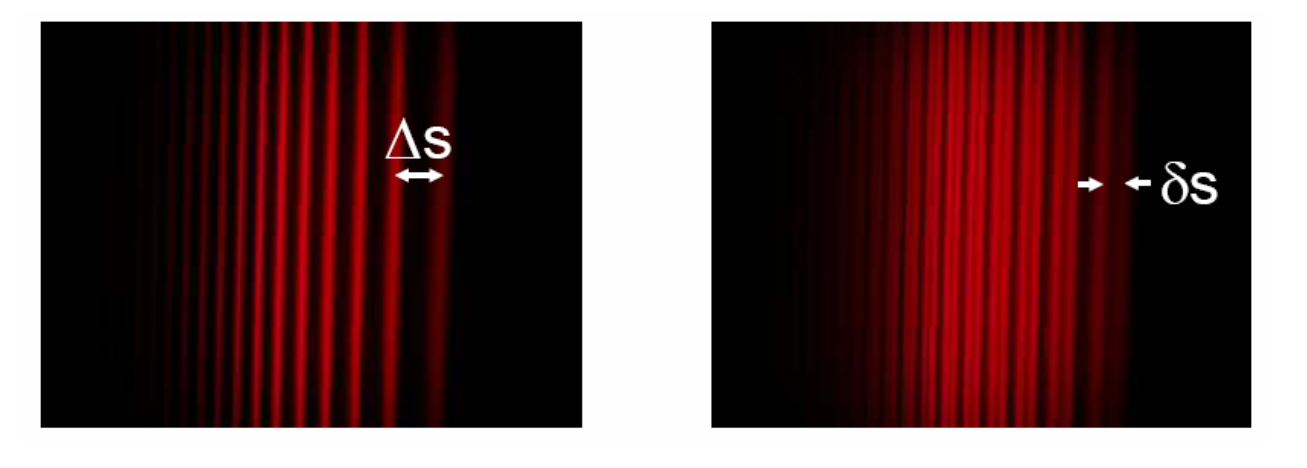
\includegraphics[width=0.7\textwidth]{pics/bsp_foto.png}
  \caption{Beispielhafte Aufnahme des Interferenzmusters der Lummer-Gehrcke Platte. %Gehrcke
  Links ohne Magnetfeld und rechts mit eingeschlatem Magnetfeld\cite{anleitung27}.}
  \label{fig: bsp_foto}
\end{figure}
\FloatBarrier
Danach wird der Elektromagnet eingeschaltet und das Magnetfeld so eingestellt, das eine Aufspaltung der
Spektrallinien erkennbar ist (vgl. Abb. \ref{fig: bsp_foto}). Da beim normalen Zeemaneffek
der Landé-Faktor konstant gleich eins ist (vgl. Tab. \ref{tab:Lande_rot}), lassen sich keine %erkennbar ist, kein Komma nach Zeemaneffekt, Landé
Übergange mit $\Delta m=0$ beobachten, denn dort ist $\Delta E=0$. Deshalb wird bei rotem Licht keine Aufspaltung
beobachtet und nur der $\sigma$- Übergang untersucht.  %es lässt sich nur keine aufspaltung beobach


Abschließend soll noch blaues Licht $\lambda=\SI{480.0}{\nm}$, welches durch den Übergang $^3S_1\leftrightarrow ^3\!\!P_1$ emittiert wird,
analysiert werden \cite{anleitung27}. Ebenso wie beim roten Licht, muss zu Beginn die Kamera justiert werden. %Beginn
Danach wird ein Bild von dem Interferenzmuster ohne Magnetfeld gemacht. Wie in der Theorie besprochen, ist der
Landé-Faktor für den anomalen Zemman-Effekt nicht mehr für jeden Zustand konstant (vgl. Tab. \ref{tab:Lande_blau}). Auf Grund dessen muss hier der Polarisationsfilter %Landé,
so eingestellt werden, dass entweder nur der $\sigma$ oder $\pi$ Übergang beobachtbar ist. Nach Einstellen des Magnetfeldes
und des Polarisationsfilters wird ein Bild von dem aufgespalteten Interferenzmuster aufgenommen. Die Durchführung wird jeweils %geschossen nicht so das passende Wort bei ner digicam :D
 für den $\sigma$ und den $\pi$ Übergang vollzogen.

Aus den einzelnen Fotos können dann die Größen $\Delta s$ und $\delta s$ (vgl. \ref{fig: bsp_foto}) abgelesen werden.
Die Werte werden dann mit dem Dispersionsgebiet in die Gleichung

\begin{equation}
  \label{eq: wellen_änderung}
  \delta \lambda=\frac{\delta s}{2\Delta s} \Delta \lambda\ua{D}
\end{equation}
eingesetz um die Wellenlängenänderung des Lichtes zu bestimmen.
Um den Übergangs-Landé-Faktor zu bestimmen, betrachtne wir die Energiediffernz, die durch die Wellenländerung gegeben ist:
\begin{equation*}
  \Delta E\ua{licht}=E(\lambda+\delta\lambda)-E(\lambda),\qquad E(\lambda)=\frac{\map{h}\map{c}}{\lambda}
\end{equation*}
Der Term $E(\lambda+\delta\lambda)$ wird durch eine Taylorentwicklung umgeschrieben zu
\begin{equation*}
  E(\lambda+\delta\lambda)\approx E(\lambda)+\frac{\partial}{\partial \lambda} E(\lambda) \delta \lambda.
\end{equation*}
Damit ergibt sich für die Energiediffenz
\begin{equation}
  \label{eq:energie_diff}
  \Delta E\ua{licht}=\frac{\partial}{\partial \lambda} E(\lambda) \delta \lambda= -\frac{\map{h}\map{c}}{\lambda^2}\delta\lambda.
\end{equation}

Durch gleichsetzen der Gleichungen \eqref{eq:energie_anomale_zemman} und \eqref{eq:energie_diff} kann dan der Übergangslandé-Faktor berechnet werden:
\begin{align}
  \Delta E\ua{licht}&=\Delta E \notag \\
   \frac{-\map{h}\map{c}}{\lambda^2}\delta\lambda & =g\map{\mu_B}B \notag \\
  \Leftrightarrow \quad g&= \frac{-\map{h}\map{c}}{\lambda^2 \map{\mu_B}B}\delta\lambda \label{eq: uebergangs_lande}.
\end{align}
